% Analysis Section
% This file contains further analysis and ablation studies

\section{Analysis}
\label{sec:analysis}

In this section, we provide further analysis of Spiral RoPE, including visualization of attention maps and ablation studies on key hyperparameters.

\subsection{Visualization of Attention Maps}

To qualitatively understand the differences between positional encoding methods, we visualize attention maps from DeiT-Base models fine-tuned at $448 \times 448$ resolution. We compare three variants: the original APE baseline, APE with axial 2D RoPE, and APE with Spiral RoPE ($K=16$).

\paragraph{Class-Token Attention.} We first visualize the class-token attention by averaging the attention weights over all heads in the last transformer layer. \cref{fig:cls_attn} shows representative examples from the ImageNet validation set. A clear progression is visible across the three methods. The APE baseline produces diffuse attention patterns, with substantial activation spread across both foreground objects and background regions. Axial RoPE improves over APE by allocating stronger attention to semantically relevant regions; however, its attention maps still exhibit noticeable residual activations in surrounding background areas and irrelevant objects. 
In contrast, Spiral RoPE yields the most object-centric and spatially coherent attention patterns, characterized by concentrated responses on the foreground objects and effective suppression of background activations. 
This advantage is particularly pronounced in multi-instance scenes, where Spiral RoPE sharply attends to multiple relevant objects, while Axial RoPE still exhibits axis-aligned artifacts and attention leakage into nearby regions.


\paragraph{Query-Token Attention.} To further examine how positional encoding influences local spatial relationships, we visualize attention patterns originating from individual patch tokens. 
\cref{fig:query_attn} shows representative examples in which the query token (marked by a red box) is located on a foreground object. 
Across all examples, APE and Axial RoPE produce attention maps that are broadly distributed across the image, with substantial activation on background regions and unrelated objects. 
In contrast, Spiral RoPE consistently produces markedly sharper and more spatially coherent attention patterns, with strong responses concentrated around the query location and semantically related regions. 
This suggests that Spiral RoPE facilitates more precise spatial alignment between query and key tokens, enabling attention to better respect local object boundaries and spatial proximity. 
We attribute this behavior to the multi-directional nature of Spiral RoPE, which encodes spatial relationships beyond axis-aligned directions and thus supports more flexible two-dimensional spatial interactions.


\begin{figure}[t]
    \centering

    \begin{subfigure}[b]{0.9\columnwidth}
        \centering
        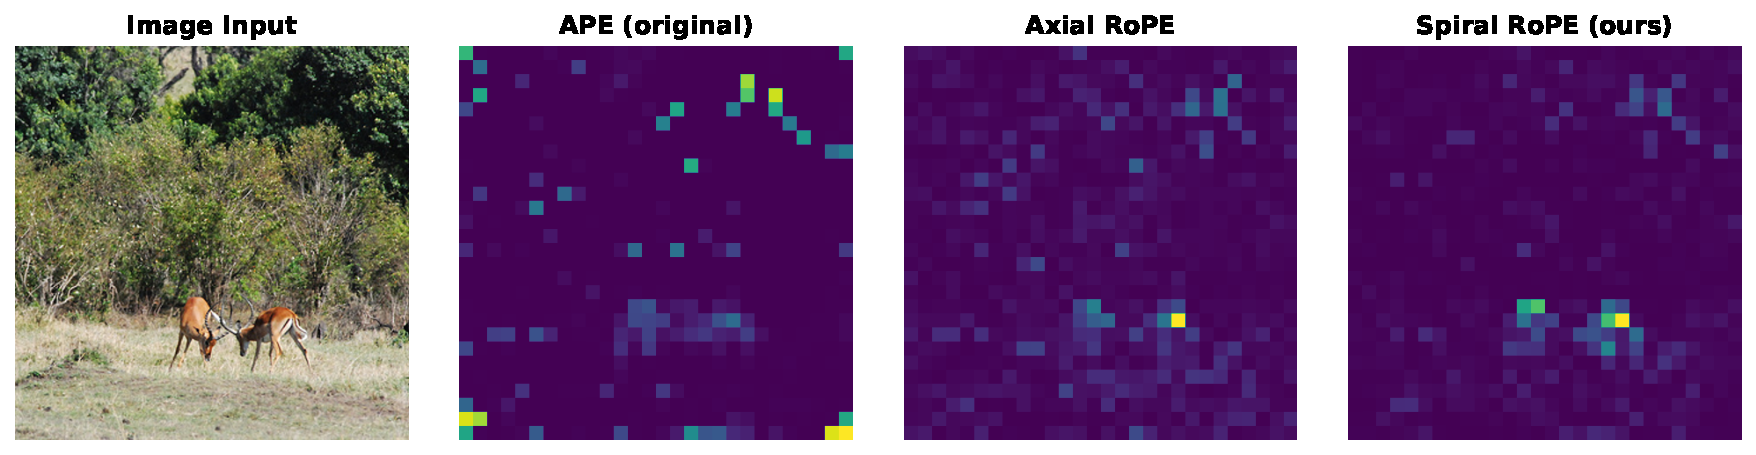
\includegraphics[width=\linewidth]{plots/ILSVRC2012_val_00029872_res448_cls_comparison_3models.pdf}
    \end{subfigure}
    \\[0.6em]

    \begin{subfigure}[b]{0.9\columnwidth}
        \centering
        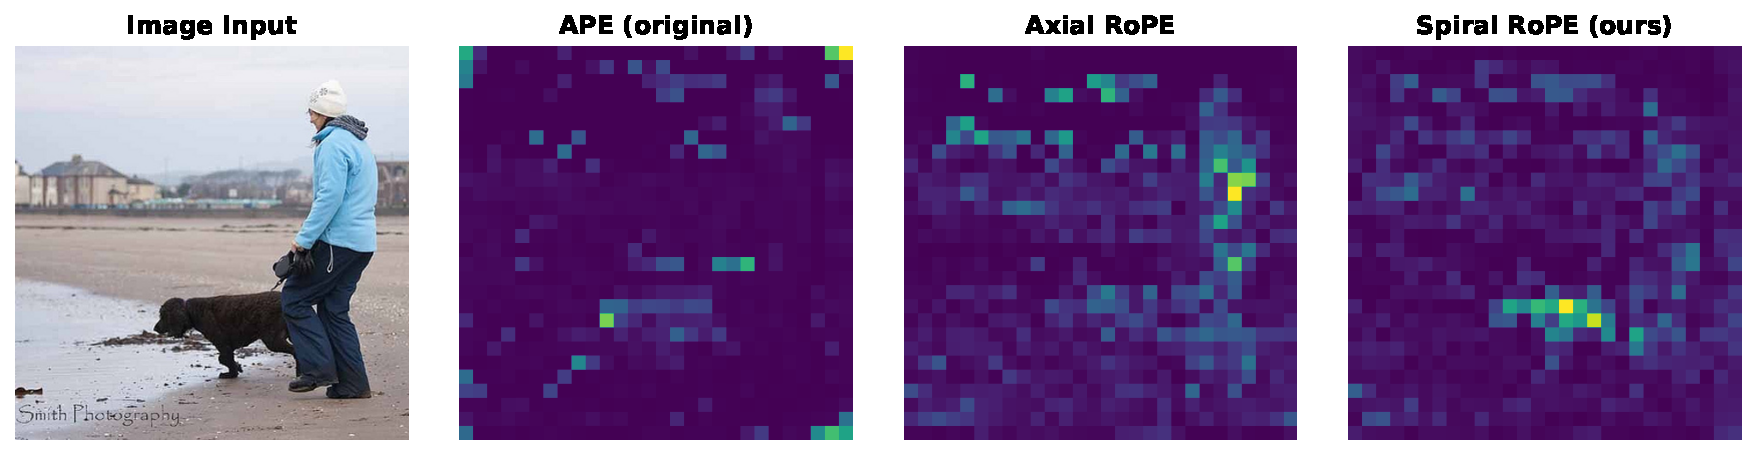
\includegraphics[width=\linewidth]{plots/ILSVRC2012_val_00030920_res448_cls_comparison_3models.pdf}
    \end{subfigure}
    \\[0.6em]

    \begin{subfigure}[b]{0.9\columnwidth}
        \centering
        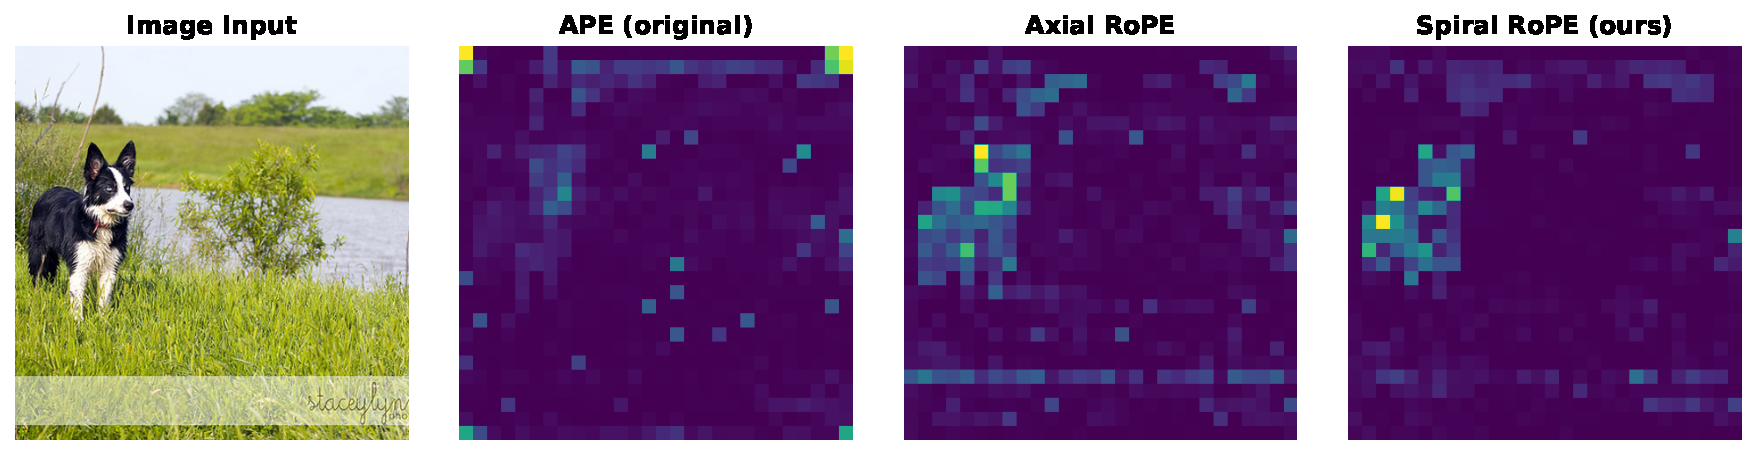
\includegraphics[width=\linewidth]{plots/ILSVRC2012_val_00046446_res448_cls_comparison_3models.pdf}
    \end{subfigure}

    \caption{\textbf{\textit{Class-token attention visualization.}} Each row shows the input image followed by attention maps from APE, Axial 2D RoPE, and Spiral RoPE. Attention is averaged over all heads in the last layer. Spiral RoPE produces more object-centric attention with cleaner background suppression compared to both counterparts.}
    \label{fig:cls_attn}
\end{figure}

\subsection{Ablation Studies}

We conduct ablation studies on the ImageNet-1k classification task using DeiT-Base at $224 \times 224$ resolution to analyze the effect of key hyperparameters in Spiral RoPE. All ablation experiments use the same training recipe as described in Section~\ref{sec:experiments:classification}, with evaluation using the final checkpoint with EMA weights and full crop.

\paragraph{Number of Directions $K$.} We first ablate the number of directions $K$ in Spiral RoPE with the frequency scaling factor fixed at 1.5. As shown in \cref{tab:ablation_k}, Spiral RoPE consistently outperforms the axial RoPE baseline (83.31\%) across all values of $K$. Increasing $K$ from 4 to 16 gradually improves accuracy, with $K=16$ achieving the best performance (83.39\%). However, further increasing $K$ to 32 slightly degrades performance (83.32\%), suggesting that excessive directional partitioning may reduce the embedding capacity per direction without providing additional benefit. Based on these results, we select $K=16$ as the default configuration for our classification experiments.

\paragraph{Frequency Scaling Factor.} We also ablate the frequency scaling factor that multiplies all base frequencies $\theta_t$ in Spiral RoPE, with $K$ fixed at 16. As shown in \cref{tab:ablation_freq}, the scaling factor has a notable impact on performance. A scaling factor of 1.0 (no scaling) achieves 83.33\%, while increasing to 1.5 yields the best result (83.39\%). However, larger scaling factors (1.75, 2.0) lead to decreased performance, likely because excessively high frequencies cause the rotations to vary too rapidly across positions, making it difficult for the model to learn stable positional relationships. We select 1.5 as the default scaling factor for our experiments.

\begin{table}[t]
    \centering
    \begin{minipage}[t]{0.48\columnwidth}
        \centering
        \caption{Ablation on the number of directions $K$.}
        \label{tab:ablation_k}
        \vspace{0.5em}
        \begin{small}
            \begin{sc}
                \begin{tabular}{lc}
                    \toprule
                    $K$ & Acc (\%) \\
                    \midrule
                    2 (Axial RoPE) & 83.31 \\
                    4 & 83.31 \\
                    8 & 83.34 \\
                    16 & \textbf{83.39} \\
                    32 & 83.32 \\
                    \bottomrule
                \end{tabular}
            \end{sc}
        \end{small}
    \end{minipage}
    \hfill
    \begin{minipage}[t]{0.48\columnwidth}
        \centering
        \caption{Ablation on the frequency scaling factor.}
        \label{tab:ablation_freq}
        \vspace{0.5em}
        \begin{small}
            \begin{sc}
                \begin{tabular}{lc}
                    \toprule
                    Scale & Acc (\%) \\
                    \midrule
                    1.00 & 83.33 \\
                    1.25 & 83.13 \\
                    1.50 & \textbf{83.39} \\
                    1.75 & 83.34 \\
                    2.00 & 83.23 \\
                    \bottomrule
                \end{tabular}
            \end{sc}
        \end{small}
    \end{minipage}
    \vskip -0.1in
\end{table}
